
%{{第三回}}{第三回}}

\chapter{金陵城起复贾雨村\\荣国府收养\textsuperscript{*}林黛玉}

*{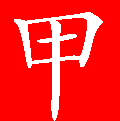
\includegraphics[width=3mm]{../Images/00002}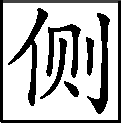
\includegraphics[width=3mm]{../Images/00011}\footnotesize \kaishu 二字触目凄凉之至!}

{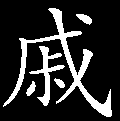
\includegraphics[width=3mm]{../Images/00005}\kaishu  我为你持戒,我为你吃斋;我为你百行百计不舒怀,我为你泪眼愁眉难解。无人处,自疑猜,生怕那慧性灵心偷改。}

{\kaishu 宝玉通灵可爱,天生有眼堪穿。万年幸一遇仙缘,从此春光美满。随时喜怒哀乐,远却离合悲欢。地久天长香影连,可意方舒心眼。}

{\kaishu 宝玉衔来,是补天之馀,落地已久,得地气收藏,因人而现。其性质内阳外阴,其形体光白温润,天生有眼可穿,故名曰宝玉,将欲得者尽皆宝爱此玉之意也。}

{\kaishu 天地循环秋复春,生生死死旧重新。君家着笔描风月,宝玉颦颦解爱人。}

却说雨村忙回头看时,不是别人,乃是当日同僚一案参革的号张如圭{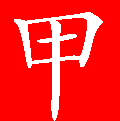
\includegraphics[width=3mm]{../Images/00002}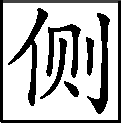
\includegraphics[width=3mm]{../Images/00011}\footnotesize \kaishu 盖言``如鬼如蜮''也,亦非正人正言。}者。他本系此地人,革职后家居,今打听得都中奏准起复旧员之信,他便四下里寻情找门路,忽遇见雨村,故忙道喜。{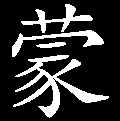
\includegraphics[width=3mm]{../Images/00006}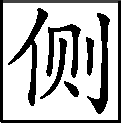
\includegraphics[width=3mm]{../Images/00011}\footnotesize \kaishu {(此)}{[}仕{]}途宦境,描写的当。}二人见了礼,张如圭便将此信告诉雨村,雨村自是欢喜,忙忙的叙了两句,{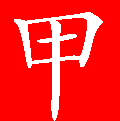
\includegraphics[width=3mm]{../Images/00002}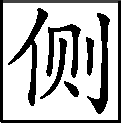
\includegraphics[width=3mm]{../Images/00011}\footnotesize \kaishu 画出心事。}遂作别各自回家。冷子兴听得此言,便忙献计,{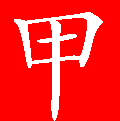
\includegraphics[width=3mm]{../Images/00002}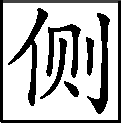
\includegraphics[width=3mm]{../Images/00011}\footnotesize \kaishu 毕肖赶热灶者。}令雨村央烦林如海,转向都中去央烦贾政。雨村领其意,作别回至馆中,忙寻邸报看真确了。{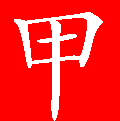
\includegraphics[width=3mm]{../Images/00002}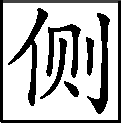
\includegraphics[width=3mm]{../Images/00011}\footnotesize \kaishu 细!}

次日,面谋之如海。如海道:``天缘凑巧,因贱荆去世,都中家岳母念及小女无人依傍教育,前已遣了男女船只来接,因小女未曾大痊,故未及行。此刻正思向蒙训教之恩未经酬报,遇此机会,岂有不尽心图报之理。但请放心,弟已预为筹画至此,已修下荐书一封,转托内兄务为周全协佐,方可稍尽弟之鄙诚,即有所费用之例,弟于内兄信中已注明白,亦不劳尊兄多虑矣。''{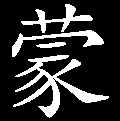
\includegraphics[width=3mm]{../Images/00006}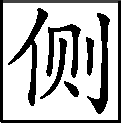
\includegraphics[width=3mm]{../Images/00011}\footnotesize \kaishu 要说正文故以此作引,且黛玉路中实无可托之人。文笔逼切得宜。}雨村一面打躬,谢不释口,一面又问:``不知令亲大人现居何职?{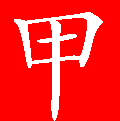
\includegraphics[width=3mm]{../Images/00002}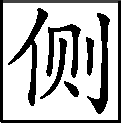
\includegraphics[width=3mm]{../Images/00011}\footnotesize \kaishu 奸险小人欺人语。}只怕晚生草率,不敢骤然入都干渎。''{{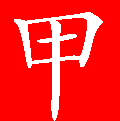
\includegraphics[width=3mm]{../Images/00002}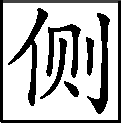
\includegraphics[width=3mm]{../Images/00011}\footnotesize \kaishu 全是假,全是诈。 }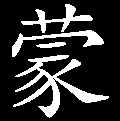
\includegraphics[width=3mm]{../Images/00006}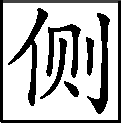
\includegraphics[width=3mm]{../Images/00011}\footnotesize \kaishu 借雨村细密心思之语,容容易易转入正文,亦是宦途人之口头心头。最妙!}如海笑道:``若论舍亲,与尊兄犹系同谱,乃荣公之孙。大内兄现袭一等将军之职,名赦,字恩侯;二内兄名政,字存周,{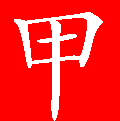
\includegraphics[width=3mm]{../Images/00002}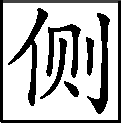
\includegraphics[width=3mm]{../Images/00011}\footnotesize \kaishu 二名二字皆颂德而来,与子兴口中作证。}现任工部员外郎,其为人谦恭厚道,大有祖父遗风,非膏粱轻薄仕宦之流,故弟方致书烦托。否则不但有污尊兄之清操,即弟亦不屑为矣。''{{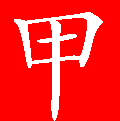
\includegraphics[width=3mm]{../Images/00002}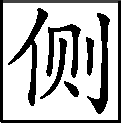
\includegraphics[width=3mm]{../Images/00011}\footnotesize \kaishu 写如海实写政老。所谓此书有``不写之写''是也。 }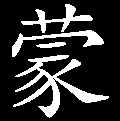
\includegraphics[width=3mm]{../Images/00006}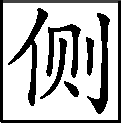
\includegraphics[width=3mm]{../Images/00011}\footnotesize \kaishu 作弊者每每偏能如此说。}雨村听了,心下方信了昨日子兴之言,于是又谢了林如海。如海乃说:``已择了出月初二日小女入都,尊兄即同路而往,岂不两便?''雨村唯唯听命,心中十分得意。如海遂打点礼物并饯行之事,雨村一一领了。

那女学生黛玉,身体大愈,原不忍弃父而往,无奈他外祖母致意务去,且兼如海说:``汝父年将半百,再无续室之意,且汝多病,年又极小,上无亲母教养,下无姊妹兄弟扶持,{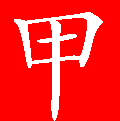
\includegraphics[width=3mm]{../Images/00002}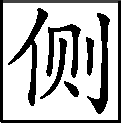
\includegraphics[width=3mm]{../Images/00011}\footnotesize \kaishu 可怜!一句一滴血,一句一滴血之文。}今依傍外祖母及舅氏姊妹去,正好减我顾盼之忧,何云不往?''黛玉听了,方洒泪拜别,{{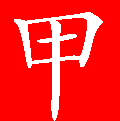
\includegraphics[width=3mm]{../Images/00002}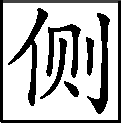
\includegraphics[width=3mm]{../Images/00011}\footnotesize \kaishu 实写黛玉。 }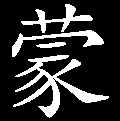
\includegraphics[width=3mm]{../Images/00006}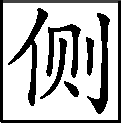
\includegraphics[width=3mm]{../Images/00011}\footnotesize \kaishu 此一段是不肯使黛玉作弃父乐为远游者。以此可见作者之心宝爱黛玉如己。}随同奶娘及荣府几个老妇人登舟而去。雨村另有一只船,带两个小童,依附黛玉而行。{{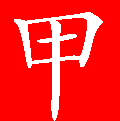
\includegraphics[width=3mm]{../Images/00002}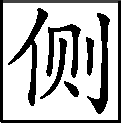
\includegraphics[width=3mm]{../Images/00011}\footnotesize \kaishu 老师依附门生,怪道今时以收纳门生为幸。 }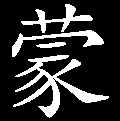
\includegraphics[width=3mm]{../Images/00006}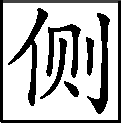
\includegraphics[width=3mm]{../Images/00011}\footnotesize \kaishu 细密如此,是大家风范。}

有日到了都中,{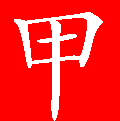
\includegraphics[width=3mm]{../Images/00002}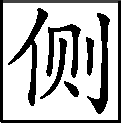
\includegraphics[width=3mm]{../Images/00011}\footnotesize \kaishu 繁中减笔。}进入神京,雨村先整了衣冠,{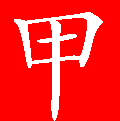
\includegraphics[width=3mm]{../Images/00002}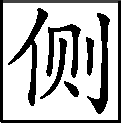
\includegraphics[width=3mm]{../Images/00011}\footnotesize \kaishu 且按下黛玉以待细写。今故先将雨村安置过一边,方起荣府中之正文也。}带了小童,{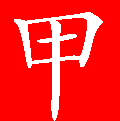
\includegraphics[width=3mm]{../Images/00002}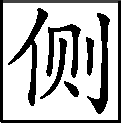
\includegraphics[width=3mm]{../Images/00011}\footnotesize \kaishu 至此渐渐好看起来也。}拿着宗侄的名帖,{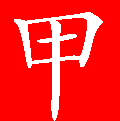
\includegraphics[width=3mm]{../Images/00002}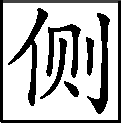
\includegraphics[width=3mm]{../Images/00011}\footnotesize \kaishu 此帖妙极,可知雨村的品行矣。}至荣府门前投了。彼时贾政已看了妹丈之书,即忙请入相会。见雨村相貌魁伟,言谈不俗,且这贾政最喜读书人,礼贤下士,拯溺济危,大有祖风,况又系妹丈致意,因此优待雨村,{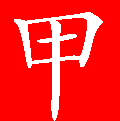
\includegraphics[width=3mm]{../Images/00002}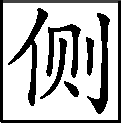
\includegraphics[width=3mm]{../Images/00011}\footnotesize \kaishu 君子可欺{[}以{]}其方也,况雨村正在王莽谦恭下士之时,虽政老亦为所惑,在作者系指东说西也。}更又不同,便竭力内中协助。题奏之日,轻轻谋{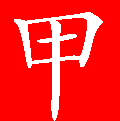
\includegraphics[width=3mm]{../Images/00002}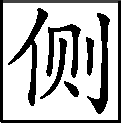
\includegraphics[width=3mm]{../Images/00011}\footnotesize \kaishu 《春秋》字法。}了一个复职候缺,不上两个月,金陵应天府缺出,便谋补{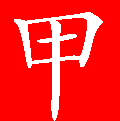
\includegraphics[width=3mm]{../Images/00002}\includegraphics[width=3mm]{../Images/00011}\footnotesize \kaishu 《春秋》字法。}了此缺,拜辞了贾政,择日到任去了。{\includegraphics[width=3mm]{../Images/00002}\includegraphics[width=3mm]{../Images/00011}\footnotesize \kaishu 因宝钗故及之,一语过至下回。}不在话下。{\includegraphics[width=3mm]{../Images/00006}\includegraphics[width=3mm]{../Images/00011}\footnotesize \kaishu 了结雨村。}

且说黛玉自那日弃舟登岸时,{\includegraphics[width=3mm]{../Images/00002}\includegraphics[width=3mm]{../Images/00011}\footnotesize \kaishu 这方是正文起头处。此后笔墨,与前两回不同。}便有荣国府打发了轿子并拉行李的车辆久候了。这黛玉常听得{{\includegraphics[width=3mm]{../Images/00002}\includegraphics[width=3mm]{../Images/00011}\footnotesize \kaishu 三字细。 }\includegraphics[width=3mm]{../Images/00006}\includegraphics[width=3mm]{../Images/00011}\footnotesize \kaishu 以``常听见''等字,省下多少笔墨。}母亲说过,他外祖母家与别家不同。他近日所见的这几个三等的仆妇,已是不凡了,何况今至其家。因此步步留心,时时在意,不肯轻意多说一句话,多行一步路,{\includegraphics[width=3mm]{../Images/00006}\includegraphics[width=3mm]{../Images/00011}\footnotesize \kaishu 颦颦故自不凡。}生恐被人耻笑了他去。{{\includegraphics[width=3mm]{../Images/00002}\includegraphics[width=3mm]{../Images/00011}\footnotesize \kaishu 写黛玉自幼之心机。 }\includegraphics[width=3mm]{../Images/00009}\includegraphics[width=3mm]{../Images/00012}\footnotesize \kaishu 黛玉自忖之语。}自上了轿,进入城中,从纱窗向外瞧了一瞧,其街市之繁华,人烟之阜盛,自与别处不同。{\includegraphics[width=3mm]{../Images/00002}\includegraphics[width=3mm]{../Images/00011}\footnotesize \kaishu 先从街市写来。}又行了半日,忽见街北蹲着两个大石狮子,三间兽头大门,门前列坐着十来个华冠丽服之人。正门却不开,只有东西两角门有人出入。正门之上有一匾,匾上大书``敕造宁国府''五个大字。{\includegraphics[width=3mm]{../Images/00002}\includegraphics[width=3mm]{../Images/00011}\footnotesize \kaishu 先写宁府,这是由东向西而来。}黛玉想道:``这是外祖母之长房了。''想着,又往西行,不多远,照样也是三间大门,方是荣国府了。却不进正门,{\includegraphics[width=3mm]{../Images/00006}\includegraphics[width=3mm]{../Images/00011}\footnotesize \kaishu 以下写{(宁)}{[}荣{]}国府第,总借黛玉一双俊眼中传来。非黛玉之眼,也不得如此细密周详。}只进了西边角门。那轿夫抬进去,走了一射之地,将转弯时,便歇下退出去了。后面婆子们已都下了轿,赶上前来。另换了三四个衣帽周全的十七八岁的小厮上来,复抬起轿子。众婆子步下围随,至一垂花门前落下。众小厮退出,众婆子上来打起轿帘,扶黛玉下轿。{\includegraphics[width=3mm]{../Images/00006}\includegraphics[width=3mm]{../Images/00011}\footnotesize \kaishu 以上写款项。}林黛玉扶着婆子的手,进了垂花门,两边是抄手游廊,当中是穿堂,当地放着一个紫檀架子大理石的大插屏。转过插屏,小小三间内厅,厅后就是后面的正房大院。正面五间上房,皆是雕梁画栋,两边穿山游廊厢房,挂着各色鹦鹉、画眉等鸟雀。台矶之上,坐着几个穿红着绿的丫鬟,一见他们来了,便忙都笑迎上来,说:``才刚老太太还念呢,可巧就来了。''{\includegraphics[width=3mm]{../Images/00002}\includegraphics[width=3mm]{../Images/00011}\footnotesize \kaishu 如见如闻,活现于纸上之笔。好看煞!}于是三四人争着打起帘栊,{\includegraphics[width=3mm]{../Images/00002}\includegraphics[width=3mm]{../Images/00011}\footnotesize \kaishu 真有是事,真有是事!}一面听得人回话:``林姑娘到了。''

黛玉方进入房时,只见两个人搀着一位鬓发如银的老母迎上来,{\includegraphics[width=3mm]{../Images/00002}\includegraphics[width=3mm]{../Images/00010}\footnotesize \kaishu 此书得力处,全是此等地方,所谓``颊上三毫''也。}黛玉便知是他外祖母。方欲拜见时,早被他外祖母一把搂入怀中,``心肝儿肉''{\includegraphics[width=3mm]{../Images/00005}\includegraphics[width=3mm]{../Images/00012}\footnotesize \kaishu 写尽天下疼女儿的神理。 \includegraphics[width=3mm]{../Images/00006}\includegraphics[width=3mm]{../Images/00011}\footnotesize \kaishu 此一段文字是天性中流出,我读时不觉泪盈双袖。}叫着大哭起来。{\includegraphics[width=3mm]{../Images/00002}\includegraphics[width=3mm]{../Images/00011}\footnotesize \kaishu 几千斤力量写此一笔。}当下地下侍立之人,无不掩面涕泣,{\includegraphics[width=3mm]{../Images/00002}\includegraphics[width=3mm]{../Images/00011}\footnotesize \kaishu 旁写一笔,更妙!}黛玉也哭个不住。{{\includegraphics[width=3mm]{../Images/00002}\includegraphics[width=3mm]{../Images/00011}\footnotesize \kaishu 自然顺写一笔。 }\includegraphics[width=3mm]{../Images/00006}\includegraphics[width=3mm]{../Images/00011}\footnotesize \kaishu 逼真。}一时众人慢慢的解劝住了,黛玉方拜见了外祖母。{\includegraphics[width=3mm]{../Images/00002}\includegraphics[width=3mm]{../Images/00010}\footnotesize \kaishu 书中正文之人,却如此写出,却是天生地设章法,不见一丝勉强。}此即冷子兴所云之史氏太君,贾赦、贾政之母也。{\includegraphics[width=3mm]{../Images/00002}\includegraphics[width=3mm]{../Images/00011}\footnotesize \kaishu 书中人目太繁,故明注一笔,使观者省眼。}当下贾母一一指与黛玉:``这是你大舅母,{\includegraphics[width=3mm]{../Images/00009}\includegraphics[width=3mm]{../Images/00012}\footnotesize \kaishu 邢氏。}这是你二舅母,{\includegraphics[width=3mm]{../Images/00009}\includegraphics[width=3mm]{../Images/00012}\footnotesize \kaishu 王氏。}这是你先珠大哥的媳妇珠大嫂。{\includegraphics[width=3mm]{../Images/00009}\includegraphics[width=3mm]{../Images/00012}\footnotesize \kaishu 李纨。}''黛玉一一拜见过。贾母又说:``请姑娘们来。今日远客才来,可以不必上学去了。''众人答应了一声,便去了两个。

不一时,只见三个奶嬷嬷并五六个丫鬟,簇拥着三个姊妹来了。{\includegraphics[width=3mm]{../Images/00002}\includegraphics[width=3mm]{../Images/00011}\footnotesize \kaishu 声势如现纸上。 \includegraphics[width=3mm]{../Images/00002}\includegraphics[width=3mm]{../Images/00010}\footnotesize \kaishu 从黛玉眼中写三人。}第一个肌肤微丰,{\includegraphics[width=3mm]{../Images/00002}\includegraphics[width=3mm]{../Images/00011}\footnotesize \kaishu 不犯宝钗。}合中身材,腮凝新荔,鼻腻鹅脂,温柔沉默,观之可亲。{\includegraphics[width=3mm]{../Images/00002}\includegraphics[width=3mm]{../Images/00011}\footnotesize \kaishu 为迎春写照。}第二个削肩细腰,{\includegraphics[width=3mm]{../Images/00002}\includegraphics[width=3mm]{../Images/00011}\footnotesize \kaishu 《洛神赋》中云``肩若削成''是也。}长挑身材,鸭蛋脸面,俊眼修眉,顾盼神飞,文彩精华,见之忘俗。{\includegraphics[width=3mm]{../Images/00002}\includegraphics[width=3mm]{../Images/00011}\footnotesize \kaishu 为探春写照。}第三个身量未足,形容尚小。{\includegraphics[width=3mm]{../Images/00002}\includegraphics[width=3mm]{../Images/00010}\footnotesize \kaishu 浑写一笔更妙!必个个写去则板矣。可笑近之小说中有一百个女子,皆是如花似玉一副脸面。}其钗环裙袄,{\includegraphics[width=3mm]{../Images/00002}\includegraphics[width=3mm]{../Images/00011}\footnotesize \kaishu 是极。}三人皆是一样的妆饰。{{\includegraphics[width=3mm]{../Images/00002}\includegraphics[width=3mm]{../Images/00011}\footnotesize \kaishu 毕肖。 }\includegraphics[width=3mm]{../Images/00006}\includegraphics[width=3mm]{../Images/00011}\footnotesize \kaishu 欲画天尊,先画{(纵)}{[}众{]}神。如此,其天尊自当另有一番高山世外的景象。}黛玉忙起身迎上来见礼,{\includegraphics[width=3mm]{../Images/00002}\includegraphics[width=3mm]{../Images/00011}\footnotesize \kaishu 此笔亦不可少。}互相厮认过,大家归坐。丫鬟们斟上茶来。不过说些黛玉之母如何得病,如何请医服药,如何送死发丧。不免贾母又伤感起来,{{\includegraphics[width=3mm]{../Images/00002}\includegraphics[width=3mm]{../Images/00011}\footnotesize \kaishu 妙! }\includegraphics[width=3mm]{../Images/00006}\includegraphics[width=3mm]{../Images/00011}\footnotesize \kaishu 层层不露,周密之至。}因说:``我这些儿女,所疼者惟有你母,今日一旦先舍我去了,连面也不能一见,今见了你,我怎么不伤心!''说着,搂了黛玉在怀,又呜咽起来。{\includegraphics[width=3mm]{../Images/00006}\includegraphics[width=3mm]{../Images/00011}\footnotesize \kaishu 不禁我也跟他哭起。}众人忙都宽慰解释,方略略止住。{\includegraphics[width=3mm]{../Images/00002}\includegraphics[width=3mm]{../Images/00011}\footnotesize \kaishu 总为黛玉自此不能别往。}

众人见黛玉年貌虽小,其举止言谈不俗,身体面庞虽怯弱不胜,{\includegraphics[width=3mm]{../Images/00002}\includegraphics[width=3mm]{../Images/00011}\footnotesize \kaishu 写美人是如此笔仗,看官怎得不叫绝称赏!}却有一段自然风流态度,{\includegraphics[width=3mm]{../Images/00002}\includegraphics[width=3mm]{../Images/00011}\footnotesize \kaishu 为黛玉写照。众人目中,只此一句足矣。 \includegraphics[width=3mm]{../Images/00002}\includegraphics[width=3mm]{../Images/00010}\footnotesize \kaishu 从众人目中写黛玉。◇草胎卉质,岂能胜物耶?想其衣裙皆不得不勉强支持者也。}便知他有不足之症。因问:``常服何药,如何不急为疗治?''黛玉笑道:``我自来是如此,从会吃饮食时便吃药,到今未断,请了多少名医修方配药,皆不见效。那一年我才三岁时,听得说{\includegraphics[width=3mm]{../Images/00002}\includegraphics[width=3mm]{../Images/00011}\footnotesize \kaishu 文字细如牛毛。}来了一个癞头和尚,{\includegraphics[width=3mm]{../Images/00002}\includegraphics[width=3mm]{../Images/00010}\footnotesize \kaishu 奇奇怪怪一至于此。通部中假借癞僧、跛道二人点明迷情幻海中有数之人也。非袭《西游》中一味无稽、至不能处便用观世音可比。}说要化我去出家,我父母固是不从。他又说:`既舍不得他,只怕他的病一生也不能好的了。若要好时,除非从此以后总不许见哭声,{\includegraphics[width=3mm]{../Images/00005}\includegraphics[width=3mm]{../Images/00012}\footnotesize \kaishu 爱哭的偏写出有人不教哭。 \includegraphics[width=3mm]{../Images/00006}\includegraphics[width=3mm]{../Images/00011}\footnotesize \kaishu 作者既以黛玉为绛珠化生,是要哭的了,反要使人先叫他不许哭。妙!}除父母之外,凡有外姓亲友之人,一概不见,方可平安了此一世。'疯疯癫癫,说了这些不经之谈,{\includegraphics[width=3mm]{../Images/00002}\includegraphics[width=3mm]{../Images/00011}\footnotesize \kaishu 是作书者自注。}也没人理他。如今还是吃人参养荣丸。''{\includegraphics[width=3mm]{../Images/00002}\includegraphics[width=3mm]{../Images/00011}\footnotesize \kaishu 人生自当自养荣卫。 \includegraphics[width=3mm]{../Images/00002}\includegraphics[width=3mm]{../Images/00010}\footnotesize \kaishu 甄英莲乃副十二钗之首,却明写癞僧一点。今黛玉为正十二钗之冠,反用暗笔。盖正十二钗人或洞悉可知,副十二钗或恐观者忽略,故写极力一提,使观者万勿稍加玩忽之意耳。}贾母道:``这正好,我这里正配丸药呢。叫他们多配一料就是了。''{\includegraphics[width=3mm]{../Images/00002}\includegraphics[width=3mm]{../Images/00011}\footnotesize \kaishu 为后菖、菱伏脉。}

一语未了,只听得后院中有人笑声{\includegraphics[width=3mm]{../Images/00002}\includegraphics[width=3mm]{../Images/00011}\footnotesize \kaishu 懦笔庸笔何能及此!}说:``我来迟了,不曾迎接远客!''{{\includegraphics[width=3mm]{../Images/00002}\includegraphics[width=3mm]{../Images/00011}\footnotesize \kaishu 第一笔,阿凤三魂六魄已被作者拘定了,后文焉得不活跳纸上?此等文字非仙助{(即)}{[}亦{]}非神助,从何而得此机括耶? \includegraphics[width=3mm]{../Images/00002}\includegraphics[width=3mm]{../Images/00010}\footnotesize \kaishu 另磨新墨,搦锐笔,特独出熙凤一人。未写其形,先使闻声,所谓``绣幡开,遥见英雄俺''也。}}黛玉纳罕道:``这些人个个皆敛声屏气,恭肃严整如此,这来者系谁,这样放诞无礼?''{{\includegraphics[width=3mm]{../Images/00002}\includegraphics[width=3mm]{../Images/00011}\footnotesize \kaishu 原有此一想。 }\includegraphics[width=3mm]{../Images/00006}\includegraphics[width=3mm]{../Images/00011}\footnotesize \kaishu 天下事不可一概而论。}心下想时,只见一群媳妇丫鬟围拥着一个人从后房门进来。这个人打扮与众姑娘不同,彩绣辉煌,恍若神妃仙子:头上戴着金丝八宝攒珠髻,绾着朝阳五凤挂珠钗,{\includegraphics[width=3mm]{../Images/00002}\includegraphics[width=3mm]{../Images/00011}\footnotesize \kaishu 头。}项上带着赤金盘螭璎珞圈,{\includegraphics[width=3mm]{../Images/00002}\includegraphics[width=3mm]{../Images/00011}\footnotesize \kaishu 颈。}裙边系着豆绿宫绦、双衡比目玫瑰佩,{\includegraphics[width=3mm]{../Images/00002}\includegraphics[width=3mm]{../Images/00011}\footnotesize \kaishu 腰。}身上穿着缕金百蝶穿花大红洋缎窄褃袄,{\includegraphics[width=3mm]{../Images/00006}\includegraphics[width=3mm]{../Images/00011}\footnotesize \kaishu 大凡能事者,多是尚奇好异,不肯泛泛同流。}外罩五彩刻丝石青银鼠褂,下着翡翠撒花洋绉裙。一双丹凤三角眼,两弯柳叶吊梢眉,{\includegraphics[width=3mm]{../Images/00006}\includegraphics[width=3mm]{../Images/00011}\footnotesize \kaishu 非如此眼,非如此眉,不得为熙凤。作者读过《麻衣相法》。}身量苗条,体格风骚,粉面含春威不露,丹唇未启笑先闻。{{\includegraphics[width=3mm]{../Images/00002}\includegraphics[width=3mm]{../Images/00011}\footnotesize \kaishu 为阿凤写照。 \includegraphics[width=3mm]{../Images/00002}\includegraphics[width=3mm]{../Images/00010}\footnotesize \kaishu 试问诸公:从来小说中可有写形追像至此者? }\includegraphics[width=3mm]{../Images/00006}\includegraphics[width=3mm]{../Images/00011}\footnotesize \kaishu 英豪本等。}黛玉连忙起身接见。贾母笑{\includegraphics[width=3mm]{../Images/00002}\includegraphics[width=3mm]{../Images/00011}\footnotesize \kaishu 阿凤一至,贾母方笑,与后文多少``笑''字作偶。}道:``你不认得他,他是我们这里有名的一个泼皮破落户儿,南省俗谓作`辣子',你只叫他`凤辣子'就是。''{\includegraphics[width=3mm]{../Images/00002}\includegraphics[width=3mm]{../Images/00011}\footnotesize \kaishu 阿凤笑声进来,老太君打诨,虽是空口传声,却是补出一向晨昏起居,阿凤于太君处承欢应候一刻不可少之人,看官勿以闲文淡文也。}黛玉正不知以何称呼,{\includegraphics[width=3mm]{../Images/00006}\includegraphics[width=3mm]{../Images/00011}\footnotesize \kaishu 想黛玉此时神情,含浑可爱。}只见众姊妹都忙告诉他道:``这是琏嫂子。''黛玉虽不识,亦曾听见母亲说过,大舅贾赦之子贾琏,娶的就是二舅母王氏之内侄女,自幼假充男儿教养的,学名叫王熙凤。{\includegraphics[width=3mm]{../Images/00002}\includegraphics[width=3mm]{../Images/00011}\footnotesize \kaishu 奇想奇文。以女子曰``学名''固奇,然此偏有学名的反倒不识字,不曰学名者反若假。}黛玉忙陪笑见礼,以``嫂''呼之。这熙凤携着黛玉的手,上下细细的打量了一回,{\includegraphics[width=3mm]{../Images/00002}\includegraphics[width=3mm]{../Images/00011}\footnotesize \kaishu 写阿凤全部传神第一笔也。}便仍送至贾母身边坐下,因笑道:``天下真有这样标致人物,我今儿才算见了!{\includegraphics[width=3mm]{../Images/00002}\includegraphics[width=3mm]{../Images/00011}\footnotesize \kaishu 这方是阿凤言语。若一味浮词套语,岂复为阿凤哉! \includegraphics[width=3mm]{../Images/00002}\includegraphics[width=3mm]{../Images/00010}\footnotesize \kaishu ``真有这样标致人物''出自凤口,黛玉丰姿可知。宜作史笔看。}况且这通身的气派,竟不像老祖宗的外孙女儿,竟是个嫡亲的孙女,{\includegraphics[width=3mm]{../Images/00002}\includegraphics[width=3mm]{../Images/00011}\footnotesize \kaishu 仍归太君,方不失《石头记》文字,且是阿凤身心之至文。}怨不得老祖宗天天口头心头,一时不忘。{{\includegraphics[width=3mm]{../Images/00002}\includegraphics[width=3mm]{../Images/00011}\footnotesize \kaishu 却是极淡之语,偏能恰投贾母之意。 }\includegraphics[width=3mm]{../Images/00006}\includegraphics[width=3mm]{../Images/00011}\footnotesize \kaishu 以``真有''``怨不得''五字,写熙凤之口头,真是机巧异常,``怨不得''三字,愚弄了多少聪明特达者。}只可怜我这妹妹这样命苦,{\includegraphics[width=3mm]{../Images/00002}\includegraphics[width=3mm]{../Images/00011}\footnotesize \kaishu 这是阿凤见黛玉正文。}怎么姑妈偏就去世了!''{\includegraphics[width=3mm]{../Images/00002}\includegraphics[width=3mm]{../Images/00011}\footnotesize \kaishu 若无这几句,便不是贾府媳妇。}说着,便用帕拭泪。贾母笑道:``我才好了,你倒来招我。{\includegraphics[width=3mm]{../Images/00002}\includegraphics[width=3mm]{../Images/00011}\footnotesize \kaishu 文字好看之极。}你妹妹远路才来,身子又弱,也才劝住了,快再休提前话!''{\includegraphics[width=3mm]{../Images/00002}\includegraphics[width=3mm]{../Images/00011}\footnotesize \kaishu 反用贾母劝,看阿凤之术亦甚矣。}这熙凤听了,忙转悲为喜道:``正是呢!我一见了妹妹,一心都在他身上了,又是欢喜,又是伤心,竟忘记了老祖宗。该打,该打!''又忙携黛玉之手,问:``妹妹几岁了?可也上过学?现吃什么药?在这里不要想家,想要什么吃的、什么顽的,只管告诉我,丫头老婆们不好了,也只管告诉我。''一面又问婆子们:``林姑娘的行李东西可搬进来了?带了几个人来?{{\includegraphics[width=3mm]{../Images/00002}\includegraphics[width=3mm]{../Images/00011}\footnotesize \kaishu 当家的人本如此,毕肖! }\includegraphics[width=3mm]{../Images/00006}\includegraphics[width=3mm]{../Images/00011}\footnotesize \kaishu 三句话不离本行,职任在兹也。}你们赶早打扫两间下房,让他们去歇歇。''

说话时,已摆了茶果上来,熙凤亲为捧茶捧果。{{\includegraphics[width=3mm]{../Images/00002}\includegraphics[width=3mm]{../Images/00011}\footnotesize \kaishu 总为黛玉眼中写出。 }\includegraphics[width=3mm]{../Images/00006}\includegraphics[width=3mm]{../Images/00011}\footnotesize \kaishu 熙凤后到,为有事,写其劳能,先为筹画,写其机巧。摇前映后之笔。}又见二舅母问他:``月钱放完了不曾?''{\includegraphics[width=3mm]{../Images/00002}\includegraphics[width=3mm]{../Images/00011}\footnotesize \kaishu 不见后文,不见此笔之妙。}熙凤道:``月钱已放完了。才刚带着人到后楼上找缎子,{\includegraphics[width=3mm]{../Images/00002}\includegraphics[width=3mm]{../Images/00011}\footnotesize \kaishu 接闲文,是本意避繁也。}找了这半日,也并没有见昨日太太说的那样,{\includegraphics[width=3mm]{../Images/00002}\includegraphics[width=3mm]{../Images/00011}\footnotesize \kaishu 却是日用家常实事。}想是太太记错了?''{\includegraphics[width=3mm]{../Images/00006}\includegraphics[width=3mm]{../Images/00011}\footnotesize \kaishu 陪笔。用得灵活,兼能形容熙凤之为人。妙心妙手,故有妙文妙口。}王夫人道:``有没有,什么要紧。''因又说道:``该随手拿出两个来,给你这妹妹去裁衣裳的,{\includegraphics[width=3mm]{../Images/00002}\includegraphics[width=3mm]{../Images/00011}\footnotesize \kaishu 仍归前文。妙妙!}等晚上想着叫人再去拿罢,可别忘了。''熙凤道:``倒是我先料着了,知道妹妹不过这两日到的,我已预备下了,{\includegraphics[width=3mm]{../Images/00002}\includegraphics[width=3mm]{../Images/00010}\footnotesize \kaishu 余知此缎阿凤并未拿出,此借王夫人之语机变欺人处耳。若信彼果拿出预备,不独被阿凤瞒过,亦且被石头瞒过了。}等太太回去过了目好送来。''{\includegraphics[width=3mm]{../Images/00002}\includegraphics[width=3mm]{../Images/00011}\footnotesize \kaishu 试看他心机。}王夫人一笑,点头不语。{{\includegraphics[width=3mm]{../Images/00002}\includegraphics[width=3mm]{../Images/00011}\footnotesize \kaishu 深取之意。 }\includegraphics[width=3mm]{../Images/00009}\includegraphics[width=3mm]{../Images/00012}\footnotesize \kaishu 很漏凤姐是个当家人。}

当下茶果已撤,贾母命两个老嬷嬷带了黛玉去见两个母舅。时贾赦之妻邢氏忙亦起身,笑道:``我带了外甥女过去,倒也便宜。''{\includegraphics[width=3mm]{../Images/00006}\includegraphics[width=3mm]{../Images/00011}\footnotesize \kaishu 以黛玉之来去候安之便,便将荣宁二府的势排描写尽矣。}贾母笑道:``正是呢,你也去罢,不必过来了。''邢夫人答应一个``是''字,遂带了黛玉与王夫人作辞,大家送至穿堂前。出了垂花门,早有众小厮们拉过一辆翠幄青紬车来。邢夫人携了黛玉坐上,{\includegraphics[width=3mm]{../Images/00009}\includegraphics[width=3mm]{../Images/00012}\footnotesize \kaishu 未识黛卿能乘此否。}众婆子们放下车帘,方命小厮们抬起,拉至宽处,方驾上驯骡,亦出了西角门,往东过了荣府正门,便入一黑油大门中,至仪门前方下来。众小厮退出,方打起车帘,邢夫人搀了黛玉的手,进入院中。黛玉度其房屋院宇,必是荣府中之花园隔断过来的。{\includegraphics[width=3mm]{../Images/00002}\includegraphics[width=3mm]{../Images/00011}\footnotesize \kaishu 黛玉之心机眼力。}进入三层仪门,果见正房厢庑游廊,悉皆小巧别致,{\includegraphics[width=3mm]{../Images/00006}\includegraphics[width=3mm]{../Images/00011}\footnotesize \kaishu 分别得历历,可想如见。}不似方才那边轩峻壮丽,且院中随处之树木山石皆有。{\includegraphics[width=3mm]{../Images/00002}\includegraphics[width=3mm]{../Images/00011}\footnotesize \kaishu 为大观园伏脉。试思荣府园今在西,后之大观园偏写在东,何不畏难之若此?}一时进入正室,早有许多盛妆丽服之姬妾丫鬟迎着。邢夫人让黛玉坐了,一面命人到外面书房去请贾赦。{\includegraphics[width=3mm]{../Images/00002}\includegraphics[width=3mm]{../Images/00011}\footnotesize \kaishu 这一句都是写贾赦,妙在全是指东击西,打草惊蛇之笔。若看其写一人即作此一人看,先生便呆了。}一时人来回说:``老爷说了:`连日身上不好,见了姑娘彼此倒伤心,{\includegraphics[width=3mm]{../Images/00002}\includegraphics[width=3mm]{../Images/00011}\footnotesize \kaishu 追魂摄魄。 \includegraphics[width=3mm]{../Images/00002}\includegraphics[width=3mm]{../Images/00010}\footnotesize \kaishu 余久不作此语矣,见此语未免一醒。}暂且不忍相见。{{\includegraphics[width=3mm]{../Images/00002}\includegraphics[width=3mm]{../Images/00011}\footnotesize \kaishu 若一见时,不独死板,且亦大失情理,亦不能有此等妙文矣。 }\includegraphics[width=3mm]{../Images/00006}\includegraphics[width=3mm]{../Images/00011}\footnotesize \kaishu 作者绣口锦心,见有见的亲切,不见有不见的亲切,直说横讲,一毫不爽。}劝姑娘不要伤心想家,{\includegraphics[width=3mm]{../Images/00006}\includegraphics[width=3mm]{../Images/00011}\footnotesize \kaishu 亦在情理之内。}跟着老太太和舅母,即同家里一样。姊妹们虽拙,大家一处伴着,亦可以解些烦闷。{\includegraphics[width=3mm]{../Images/00002}\includegraphics[width=3mm]{../Images/00011}\footnotesize \kaishu 赦老亦能作此语,叹叹!}或有委屈之处,只管说得,不要外道才是。'''黛玉忙站起来,一一听了。再坐一刻,便告辞。那邢夫人苦留吃过晚饭去,黛玉笑回道:``舅母爱惜赐饭,原不应辞,只是还要过去拜见二舅舅,恐领了赐去不恭,{{\includegraphics[width=3mm]{../Images/00002}\includegraphics[width=3mm]{../Images/00011}\footnotesize \kaishu 得体。 }\includegraphics[width=3mm]{../Images/00006}\includegraphics[width=3mm]{../Images/00011}\footnotesize \kaishu 黛玉之为人,必当有如此身分。}异日再领,未为不可。望舅母容谅。''邢夫人听说,笑道:``这倒是了。''遂命两三个嬷嬷,用方才的车好生送了过去,于是黛玉告辞。邢夫人送至仪门前,又嘱咐众人几句,{\includegraphics[width=3mm]{../Images/00006}\includegraphics[width=3mm]{../Images/00011}\footnotesize \kaishu 又嘱咐了几句,方是舅母的本等。}眼看着车去了方回来。

一时黛玉进入荣府,下了车。众嬷嬷引着,便往东转弯,穿过一个东西的穿堂,{\includegraphics[width=3mm]{../Images/00002}\includegraphics[width=3mm]{../Images/00011}\footnotesize \kaishu 这一个穿堂是贾母正房之南者,凤姐处所通者则是贾母正房之北。}向南大厅之后,仪门内大院落,上面五间大正房,两边厢房鹿顶耳房钻山,四通八达,轩昂壮丽,比贾母处不同。黛玉便知这方是正经正内室,一条大甬路,直接出大门的。进入堂屋中,抬头迎面先看见一个赤金九龙青地大匾,匾上写着斗大三个字,是``荣禧堂'',{\includegraphics[width=3mm]{../Images/00006}\includegraphics[width=3mm]{../Images/00011}\footnotesize \kaishu 真是荣国府。}后有一行小字:``某年月日,书赐荣国公贾源。''又有``万几宸翰之宝''。大紫檀雕螭案上,设着三尺来高青绿古铜鼎,悬着待漏随朝墨龙大画,一边是金蜼彝,{\includegraphics[width=3mm]{../Images/00002}\includegraphics[width=3mm]{../Images/00011}\footnotesize \kaishu 蜼,音垒。周器也。}一边是玻璃\includegraphics[width=4mm]{../Images/00013}。{{{\includegraphics[width=3mm]{../Images/00002}\includegraphics[width=3mm]{../Images/00011}\footnotesize \kaishu }{\includegraphics[width=3mm]{../Images/00014},音海。盛酒之大器也。}}}地下两溜十六张楠木交椅。又有一副对联,乃是乌木联牌,镶着錾银的字迹,{\includegraphics[width=3mm]{../Images/00002}\includegraphics[width=3mm]{../Images/00011}\footnotesize \kaishu 雅而丽,富而文。}道是:

座上珠玑昭日月,堂前黼黻焕烟霞。{\includegraphics[width=3mm]{../Images/00002}\includegraphics[width=3mm]{../Images/00012}\footnotesize \kaishu 实贴。}

下面一行小字,道是:同乡世教弟勋袭东安郡王穆莳拜手书。{\includegraphics[width=3mm]{../Images/00002}\includegraphics[width=3mm]{../Images/00011}\footnotesize \kaishu 先虚陪一笔。}

原来王夫人时常居坐宴息,亦不在这正室,{\includegraphics[width=3mm]{../Images/00002}\includegraphics[width=3mm]{../Images/00011}\footnotesize \kaishu 黛玉由正室一段而来,是为拜见政老耳,故进东房。}只在这正室东边的三间耳房内。{\includegraphics[width=3mm]{../Images/00002}\includegraphics[width=3mm]{../Images/00011}\footnotesize \kaishu 若见王夫人,直写引至东廊小正室内矣。}于是老嬷嬷引黛玉进东房门来。临窗大炕上铺着猩红洋罽,正面设着大红金钱蟒靠背,石青金钱蟒引枕,秋香色金钱蟒大条褥。两边设一对梅花式洋漆小几。左边几上文王鼎、匙箸、香盒,右边几上汝窑美人觚------内插着时鲜花卉,并茗碗、唾壶等物。地下面西一溜四张椅上,都搭着银红撒花椅搭,底下四副脚踏。椅子两边,也有一对高几,几上茗碗花瓶俱备。其馀陈设,自不必细说。{\includegraphics[width=3mm]{../Images/00002}\includegraphics[width=3mm]{../Images/00011}\footnotesize \kaishu 此不过略叙荣府家常之礼数,特使黛玉一识阶级座次耳,馀则繁。}老嬷嬷们让黛玉炕上坐,炕沿上却也有两个锦褥对设,黛玉度其位次,便不上炕,只向东边椅子上坐了。{\includegraphics[width=3mm]{../Images/00002}\includegraphics[width=3mm]{../Images/00011}\footnotesize \kaishu 写黛玉心意。}本房内的丫鬟忙捧上茶来。黛玉一面吃茶,一面打量这些丫鬟们,{\includegraphics[width=3mm]{../Images/00006}\includegraphics[width=3mm]{../Images/00011}\footnotesize \kaishu 借黛玉眼写三等使婢。}妆饰衣裙,举止行动,果亦与别家不同。

茶未吃了,只见一个穿红绫袄、青缎掐牙背心的丫鬟{\includegraphics[width=3mm]{../Images/00002}\includegraphics[width=3mm]{../Images/00011}\footnotesize \kaishu 金乎?玉乎?}走来笑说道:``太太说,请姑娘到那边坐罢。''{\includegraphics[width=3mm]{../Images/00006}\includegraphics[width=3mm]{../Images/00011}\footnotesize \kaishu 唤去见,方是舅母,方是大家风范。}老嬷嬷听了,于是又引黛玉出来,到了东廊三间小正房内。正面炕上横设一张炕桌,桌上磊着书籍茶具,{\includegraphics[width=3mm]{../Images/00002}\includegraphics[width=3mm]{../Images/00011}\footnotesize \kaishu 伤心笔,堕泪笔。}靠东壁面西设着半旧青缎靠背引枕。王夫人却坐在西边下首,亦是半旧青缎靠背坐褥。见黛玉来了,便往东让。黛玉心中料定这是贾政之位。{\includegraphics[width=3mm]{../Images/00002}\includegraphics[width=3mm]{../Images/00011}\footnotesize \kaishu 写黛玉心到眼到,伧夫但云为贾府叙坐位,岂不可笑?}因见挨炕一溜三张椅子上,也搭着半旧的{\includegraphics[width=3mm]{../Images/00002}\includegraphics[width=3mm]{../Images/00011}\footnotesize \kaishu 三字有神。}弹墨椅袱,{\includegraphics[width=3mm]{../Images/00002}\includegraphics[width=3mm]{../Images/00011}\footnotesize \kaishu 此处则一色旧的,可知前正室中亦非家常之用度也。可笑近之小说中,不论何处,则曰商彝周鼎、绣幕珠帘、孔雀屏、芙蓉褥等样字眼。}黛玉便向椅上坐了。{\includegraphics[width=3mm]{../Images/00002}\includegraphics[width=3mm]{../Images/00010}\footnotesize \kaishu 近闻一俗笑语云:一庄农人进京回家,众人问曰:``你进京去可见些个世面否?''庄人曰:``连皇帝老爷都见了。''众罕然问曰:``皇帝如何景况?''庄人曰:``皇帝左手拿一金元宝,右手拿一银元宝,马上捎着一口袋人参,行动人参不离口。一时要屙屎了,连擦屁股都用的是鹅黄缎子,所以京中掏茅厕的人都富贵无比。''试思凡稗官写富贵字眼者,悉皆庄农进京之一流也。盖此时彼实未身经目睹,所言皆在情理之外焉。◇又如人嘲作诗者亦往往爱说富丽话,故有``胫骨变成金玳瑁,眼睛嵌作碧琉璃''之诮。余自是评《石头记》,非鄙薄前人也。}王夫人再四携他上炕,他方挨王夫人坐了。王夫人因说:``你舅舅今日斋戒去了,{\includegraphics[width=3mm]{../Images/00002}\includegraphics[width=3mm]{../Images/00011}\footnotesize \kaishu 点缀宦途。}再见罢。{\includegraphics[width=3mm]{../Images/00002}\includegraphics[width=3mm]{../Images/00011}\footnotesize \kaishu 赦老不见,又写政老。政老又不能见,是重不见重,犯不见犯。作者惯用此等章法。}只是有一句话嘱咐你:你三个姊妹倒都极好,以后一处念书认字学针线,或是偶一顽笑,都有尽让的。但我不放心的最是一件:{\includegraphics[width=3mm]{../Images/00006}\includegraphics[width=3mm]{../Images/00011}\footnotesize \kaishu 王夫人嘱咐与邢夫人嘱咐,似同{(的)}{[}而{]}迥异。儿女累心,我欲代伊哭诉一面愁苦。}我有一个孽根祸胎,{\includegraphics[width=3mm]{../Images/00002}\includegraphics[width=3mm]{../Images/00011}\footnotesize \kaishu 四字是血泪盈面,不得已无奈何而下。四字是作者痛哭。}是这家里的`混世魔王',{\includegraphics[width=3mm]{../Images/00002}\includegraphics[width=3mm]{../Images/00011}\footnotesize \kaishu 与``绛洞花王''为对看。}今日因庙里还愿去了,{\includegraphics[width=3mm]{../Images/00002}\includegraphics[width=3mm]{../Images/00011}\footnotesize \kaishu 是富贵公子。}尚未回来,晚间你看见便知。你只以后不要睬他,你这些姊妹都不敢沾惹他的。''

黛玉亦常听得母亲说过,二舅母生的有个表兄,乃衔玉而诞,顽劣异常,{\includegraphics[width=3mm]{../Images/00002}\includegraphics[width=3mm]{../Images/00011}\footnotesize \kaishu 与甄家子恰对。}极恶读书,{\includegraphics[width=3mm]{../Images/00002}\includegraphics[width=3mm]{../Images/00011}\footnotesize \kaishu 是极恶每日``诗云''``子曰''的读书。}最喜在内帏厮混,外祖母又极溺爱,无人敢管。今见王夫人如此说,便知说的是这表兄了。{\includegraphics[width=3mm]{../Images/00002}\includegraphics[width=3mm]{../Images/00010}\footnotesize \kaishu 这是一段反衬章法。黛玉心用``猜度蠢物''等句对着去,方不失作者本旨。}因陪笑道:``舅母说的,可是衔玉所生的这位哥哥?在家时亦曾听见母亲常说,{\includegraphics[width=3mm]{../Images/00006}\includegraphics[width=3mm]{../Images/00011}\footnotesize \kaishu 有曾听得,所以闻言便知,不必用心搜求了。}这位哥哥比我大一岁,小名就唤宝玉,{\includegraphics[width=3mm]{../Images/00002}\includegraphics[width=3mm]{../Images/00011}\footnotesize \kaishu 以黛玉道宝玉名,方不失正文。}虽{\includegraphics[width=3mm]{../Images/00002}\includegraphics[width=3mm]{../Images/00011}\footnotesize \kaishu ``虽''字是有情字,宿根而发,勿得泛泛看过。}极憨顽,说在姊妹情中极好的。{\includegraphics[width=3mm]{../Images/00006}\includegraphics[width=3mm]{../Images/00011}\footnotesize \kaishu 黛玉口中心中早中此。}况我来了,自然只和姊妹同处,兄弟们自是别院另室的,{\includegraphics[width=3mm]{../Images/00002}\includegraphics[width=3mm]{../Images/00011}\footnotesize \kaishu 又登开一笔,妙妙!}岂得去沾惹之理?''{\includegraphics[width=3mm]{../Images/00006}\includegraphics[width=3mm]{../Images/00011}\footnotesize \kaishu 用黛玉反衬一句,更有深味。}王夫人笑道:``你不知道原故。他与别人不同,自幼因老太太疼爱,原系同姊妹一处娇养惯了的。{\includegraphics[width=3mm]{../Images/00002}\includegraphics[width=3mm]{../Images/00011}\footnotesize \kaishu 此一笔收回,是明通部同处原委也。}若姊妹们有日不理他,他倒还安静些,纵然他没趣,不过出了二门,背地里拿着他的两三个小幺儿出气,咕唧一会子就完了。{\includegraphics[width=3mm]{../Images/00002}\includegraphics[width=3mm]{../Images/00011}\footnotesize \kaishu 这可是宝玉本性真情,前四十九字迥异之批今始方知。盖小人口碑累累如是。是是非非任尔口角,大都皆然。}若这一日姊妹们和他多说一句话,他心里一乐,便生出多少事来。所以嘱咐你别睬他。他嘴里一时甜言蜜语,一时有天无日,一时又疯疯傻傻,只休信他。''{\includegraphics[width=3mm]{../Images/00002}\includegraphics[width=3mm]{../Images/00010}\footnotesize \kaishu 不写黛玉眼中之宝玉,却先写黛玉心中已早有一宝玉矣,幻妙之至!自冷子兴口中之后,余已极思欲一见,及今尚未得见,狡猾之至! }

黛玉一一的都答应着。{\includegraphics[width=3mm]{../Images/00006}\includegraphics[width=3mm]{../Images/00011}\footnotesize \kaishu 客居之苦,在有意无意中写来。}只见一个丫鬟来回:``老太太那里传晚饭了。''王夫人忙携了黛玉从后房门{\includegraphics[width=3mm]{../Images/00002}\includegraphics[width=3mm]{../Images/00011}\footnotesize \kaishu 后房门。}由后廊{\includegraphics[width=3mm]{../Images/00002}\includegraphics[width=3mm]{../Images/00011}\footnotesize \kaishu 是正房后廊也。}往西,出了角门,{\includegraphics[width=3mm]{../Images/00002}\includegraphics[width=3mm]{../Images/00011}\footnotesize \kaishu 这是正房后西界墙角门。}是一条南北宽夹道。南边是倒座三间小小的抱厦厅,北边立着一个粉油大影壁,后有一半大门,小小一所房宇。王夫人笑指向黛玉道:``这是你凤姐姐的屋子,回来你好往这里找他来,{\includegraphics[width=3mm]{../Images/00006}\includegraphics[width=3mm]{../Images/00011}\footnotesize \kaishu 灵活。无一漏空。}少什么东西,你只管和他说就是了。''这院门上也有{\includegraphics[width=3mm]{../Images/00002}\includegraphics[width=3mm]{../Images/00011}\footnotesize \kaishu 二字是他处不写之写也。}四五个才总角的小厮,都垂手侍立。王夫人遂携黛玉穿过一个东西穿堂,{\includegraphics[width=3mm]{../Images/00002}\includegraphics[width=3mm]{../Images/00010}\footnotesize \kaishu 这正是贾母正室后之穿堂也,与前穿堂是一带之屋,中一带乃贾母之下室也。记清。}便是贾母的后院了。{\includegraphics[width=3mm]{../Images/00002}\includegraphics[width=3mm]{../Images/00011}\footnotesize \kaishu 写得清,一丝不错。}于是,进入后房门,已有多人在此伺候,见王夫人来了,方安设桌椅。{\includegraphics[width=3mm]{../Images/00002}\includegraphics[width=3mm]{../Images/00011}\footnotesize \kaishu 不是待王夫人用膳,是恐使王夫人有失侍膳之礼耳。}贾珠之妻李氏捧饭,熙凤安箸,王夫人进羹。{\includegraphics[width=3mm]{../Images/00006}\includegraphics[width=3mm]{../Images/00011}\footnotesize \kaishu 大人家规矩礼法。}贾母正面榻上独坐,两边四张空椅,熙凤忙拉了黛玉在左边第一张椅上坐了,黛玉十分推让。贾母笑道:``你舅母和嫂子们不在这里吃饭。你是客,原应如此坐的。''黛玉方告了座,坐了。贾母命王夫人坐了。迎春姊妹三个告了座,方上来。迎春便坐右手第一,探春左第二,惜春右第二。旁边丫鬟执着拂尘、漱盂、巾帕。李、凤二人立于案旁布让。外间伺候之媳妇丫鬟虽多,却连一声咳嗽不闻。寂然饭毕,各有丫鬟用小茶盘捧上茶来。{\includegraphics[width=3mm]{../Images/00006}\includegraphics[width=3mm]{../Images/00011}\footnotesize \kaishu 作者非身履其境过,不能如此细密完足。}当日林如海教女以惜福养身,云饭后务待饭粒咽尽,过一时再吃茶,方不伤脾胃。{\includegraphics[width=3mm]{../Images/00002}\includegraphics[width=3mm]{../Images/00011}\footnotesize \kaishu 夹写如海一派书气,最妙!}今黛玉见了这里许多事情不合家中之式,不得不随的,少不得一一的改过来,{\includegraphics[width=3mm]{../Images/00006}\includegraphics[width=3mm]{../Images/00011}\footnotesize \kaishu 幼而学,壮而行者常情。有不得已,行权达变,多至于失守者,亦千古同慨,诚可悲夫!}因而接了茶。早见人又捧过漱盂来,黛玉也照样漱了口。然后盥手毕,又捧上茶来,方是吃的茶。{\includegraphics[width=3mm]{../Images/00002}\includegraphics[width=3mm]{../Images/00011}\footnotesize \kaishu 总写黛玉以后之事,故只以此一件小事略为一表也。 \includegraphics[width=3mm]{../Images/00002}\includegraphics[width=3mm]{../Images/00010}\footnotesize \kaishu 余看至此,故想日前所阅``王敦初尚公主,登厕时不知塞鼻用枣,敦辄取而啖之,早为宫人鄙诮多矣''。今黛玉若不漱此茶,或饮一口,不为荣婢所诮乎?观此则知黛玉平生之心思过人。}贾母便说:``你们去罢,让我们自在说话儿。''王夫人听了,忙起身,又说了两句闲话,方引李、凤二人去了。贾母因问黛玉念何书。黛玉道:``只刚念了《四书》。''{\includegraphics[width=3mm]{../Images/00002}\includegraphics[width=3mm]{../Images/00011}\footnotesize \kaishu 好极!稗官专用``腹隐五车书''者来看。}黛玉又问姊妹们读何书。贾母道:``读的是什么书!不过是认得两个字,不是睁眼的瞎子罢了。''

一语未了,只听院外一阵脚步响,{\includegraphics[width=3mm]{../Images/00002}\includegraphics[width=3mm]{../Images/00011}\footnotesize \kaishu 与阿凤之来相映而不相犯。}丫鬟进来笑道:``宝玉来了!''{{\includegraphics[width=3mm]{../Images/00002}\includegraphics[width=3mm]{../Images/00011}\footnotesize \kaishu 余为一乐。 }\includegraphics[width=3mm]{../Images/00006}\includegraphics[width=3mm]{../Images/00011}\footnotesize \kaishu 形容出姣养,神。}黛玉心中正疑惑着:``这个宝玉,不知是怎生个惫懒人物、懵懂顽童?{{\includegraphics[width=3mm]{../Images/00002}\includegraphics[width=3mm]{../Images/00011}\footnotesize \kaishu 文字不反,不见正文之妙,似此应从《国策》得来。 }\includegraphics[width=3mm]{../Images/00006}\includegraphics[width=3mm]{../Images/00011}\footnotesize \kaishu 从黛玉口中故反一句,则下文更觉生色。}倒不见那蠢物也罢了。\href{../Text/part0007_split_000.html\#lnkback_1_a}{\textsuperscript{①}}''{\includegraphics[width=3mm]{../Images/00002}\includegraphics[width=3mm]{../Images/00011}\footnotesize \kaishu 这蠢物不是那蠢物,却有个极蠢之物相待。妙极!}心中正想着,忽见丫鬟话未报完,已进来了一个年轻\href{../Text/part0007_split_000.html\#lnkback_2_a}{\textsuperscript{②}}公子:头上戴着束发嵌宝紫金冠,齐眉勒着二龙抢珠金抹额,穿一件二色金百蝶穿花大红箭袖,束着五彩丝攒花结长穗宫绦,外罩石青起花八团倭缎排穗褂,登着青缎粉底小朝靴。面若中秋之月,{\includegraphics[width=3mm]{../Images/00002}\includegraphics[width=3mm]{../Images/00010}\footnotesize \kaishu 此非套``满月'',盖人生有面扁而青白色者,则皆可谓之秋月也。用``满月''者不知此意。}色如春晓之花。{\includegraphics[width=3mm]{../Images/00002}\includegraphics[width=3mm]{../Images/00010}\footnotesize \kaishu ``少年色嫩不坚牢'',以及``非夭即贫''之语,余犹在心。今阅至此,放声一哭。}鬓如刀裁,眉如墨画,眼似桃瓣,睛若秋波。虽怒时而若笑,即嗔视而有情。{\includegraphics[width=3mm]{../Images/00002}\includegraphics[width=3mm]{../Images/00011}\footnotesize \kaishu 真真写杀。}项上金螭璎珞,又有一根五色丝绦,系着一块美玉。黛玉一见,{\includegraphics[width=3mm]{../Images/00005}\includegraphics[width=3mm]{../Images/00012}\footnotesize \kaishu 写宝玉只是宝玉,写黛玉只是黛玉,从中用黛玉一惊宝玉之面善等字,文气自然笼就,要分开不得了。}便吃一大惊,{\includegraphics[width=3mm]{../Images/00002}\includegraphics[width=3mm]{../Images/00011}\footnotesize \kaishu 怪甚。}心下想道:``好生奇怪,倒像在那里见过的一般,{\includegraphics[width=3mm]{../Images/00006}\includegraphics[width=3mm]{../Images/00011}\footnotesize \kaishu 此一惊,方下文之留连缠绵,不为孟浪,不是淫邪。}何等眼熟到如此!''{\includegraphics[width=3mm]{../Images/00002}\includegraphics[width=3mm]{../Images/00011}\footnotesize \kaishu 正是。想必在灵河岸上三生石畔曾见过。}

只见这宝玉向贾母请了安,贾母便命:``去见你娘来。''宝玉即转身去了。一时回来,再看,已换了冠带:头上周围一转的短发,都结成了小辫,红丝结束,共攒至顶中胎发,总编一根大辫,黑亮如漆,从顶至梢,一串四颗大珠,用金八宝坠角,身上穿着银红撒花半旧大袄,仍旧带着项圈、宝玉、寄名锁、护身符等物,下面半露松花撒花绫裤腿,锦边弹墨袜,厚底大红鞋。越显得面如敷粉,唇若施脂;转盼多情,语言常笑。天然一段风骚,全在眉梢;平生万种情思,悉堆眼角。{\includegraphics[width=3mm]{../Images/00006}\includegraphics[width=3mm]{../Images/00011}\footnotesize \kaishu 总是写宝玉,总是为下文留地步。}看其外貌最是极好,却难知其底细。后人有《西江月》二词,批这宝玉极恰,{\includegraphics[width=3mm]{../Images/00002}\includegraphics[width=3mm]{../Images/00010}\footnotesize \kaishu 二词更妙。最可厌野史``貌如潘安''``才如子建''等语。}其词曰:

无故寻愁觅恨,有时似傻如狂。纵然生得好皮囊,腹内原来草莽。  潦倒不通世务,愚顽怕读文章。行为偏僻性乖张,那管世人诽谤!

富贵不知乐业,贫穷难耐凄凉。可怜辜负好韶光,于国于家无望。  天下无能第一,古今不肖无双。寄言纨袴与膏粱:莫效此儿形状!{{\includegraphics[width=3mm]{../Images/00002}\includegraphics[width=3mm]{../Images/00010}\footnotesize \kaishu 末二语最要紧。只是纨绔膏粱,亦未必不见笑我玉卿。可知能效一二者,亦必不是蠢然纨绔矣。 }\includegraphics[width=3mm]{../Images/00005}\includegraphics[width=3mm]{../Images/00012}\footnotesize \kaishu 纨袴膏粱,此儿形状有意思。当设想其像,合宝玉之来历同看,方不被作者愚弄。}

贾母因笑道:``外客未见,就脱了衣裳,还不去见你妹妹!''宝玉早已看见多了一个姊妹,便料定是林姑母之女,忙来作揖。厮见毕归坐,细看形容,{\includegraphics[width=3mm]{../Images/00002}\includegraphics[width=3mm]{../Images/00010}\footnotesize \kaishu 又从宝玉目中细写一黛玉,直画一美人图。}与众各别:两弯似蹙非蹙罥烟眉,{\includegraphics[width=3mm]{../Images/00002}\includegraphics[width=3mm]{../Images/00011}\footnotesize \kaishu 奇眉妙眉,奇想妙想。}一双似泣非泣含露目。\href{../Text/part0007_split_000.html\#lnkback_3_a}{\textsuperscript{③}}{\includegraphics[width=3mm]{../Images/00002}\includegraphics[width=3mm]{../Images/00011}\footnotesize \kaishu 奇目妙目,奇想妙想。}态生两靥之愁,娇袭一身之病。泪光点点,娇喘微微。闲静时如娇花照水,行动处似弱柳扶风。{\includegraphics[width=3mm]{../Images/00002}\includegraphics[width=3mm]{../Images/00011}\footnotesize \kaishu 至此八句是宝玉眼中。}心较比干多一窍,{{\includegraphics[width=3mm]{../Images/00002}\includegraphics[width=3mm]{../Images/00011}\footnotesize \kaishu 此一句是宝玉心中。 \includegraphics[width=3mm]{../Images/00002}\includegraphics[width=3mm]{../Images/00010}\footnotesize \kaishu 更奇妙之至!多一窍固是好事,然未免偏僻了,所谓``过犹不及''也。 }\includegraphics[width=3mm]{../Images/00006}\includegraphics[width=3mm]{../Images/00011}\footnotesize \kaishu 写黛玉,也是为下文留地步。}病如西子胜三分。{\includegraphics[width=3mm]{../Images/00002}\includegraphics[width=3mm]{../Images/00011}\footnotesize \kaishu 此十句定评,直抵一赋。 \includegraphics[width=3mm]{../Images/00002}\includegraphics[width=3mm]{../Images/00010}\footnotesize \kaishu 不写衣裙妆饰,正是宝玉眼中不屑之物,故不曾看见。黛玉之举止容貌,亦是宝玉眼中看、心中评。若不是宝玉,断不能知黛玉终是何等品貌。}宝玉看罢,因笑{\includegraphics[width=3mm]{../Images/00002}\includegraphics[width=3mm]{../Images/00010}\footnotesize \kaishu 黛玉见宝玉写一``惊''字,宝玉见黛玉写一``笑''字,一存于中,一发乎外,可见文于下笔必推敲的准稳,方才用字。}道:{\includegraphics[width=3mm]{../Images/00002}\includegraphics[width=3mm]{../Images/00011}\footnotesize \kaishu 看他第一句是何话。}``这个妹妹我曾见过的。''{\includegraphics[width=3mm]{../Images/00002}\includegraphics[width=3mm]{../Images/00011}\footnotesize \kaishu 疯话。与黛玉同心,却是两样笔墨。观此则知玉卿心中有则说出,一毫宿滞皆无。}贾母笑道:``可又是胡说,你又何曾见过他?''宝玉笑道:``虽然未曾见过他,然我看着面善,心里就算是旧相识,{{\includegraphics[width=3mm]{../Images/00002}\includegraphics[width=3mm]{../Images/00011}\footnotesize \kaishu 一见便作如是语,宜乎王夫人谓之疯疯傻傻也。 }\includegraphics[width=3mm]{../Images/00006}\includegraphics[width=3mm]{../Images/00011}\footnotesize \kaishu 世人得遇相好者,每曰一见如故,与此一意。}今日只作远别重逢,未为不可。''{\includegraphics[width=3mm]{../Images/00002}\includegraphics[width=3mm]{../Images/00011}\footnotesize \kaishu 妙极奇语。全作如是等语,{[}焉{]}怪人谓曰痴狂。 \includegraphics[width=3mm]{../Images/00002}\includegraphics[width=3mm]{../Images/00011}\footnotesize \kaishu 作小儿语瞒过世人亦可。}贾母笑道:``更好,更好。若如此,更相和睦了。''{\includegraphics[width=3mm]{../Images/00002}\includegraphics[width=3mm]{../Images/00011}\footnotesize \kaishu 亦是真话。}宝玉便走近黛玉身边坐下,又细细打量一番,{{\includegraphics[width=3mm]{../Images/00002}\includegraphics[width=3mm]{../Images/00011}\footnotesize \kaishu 与黛玉两次打量一对。 }\includegraphics[width=3mm]{../Images/00006}\includegraphics[width=3mm]{../Images/00011}\footnotesize \kaishu 姣惯处如画。如此亲近,而黛玉之灵心巧性,能不被其缚住,反不是性理。文从宽缓中写来,妙!}因问:``妹妹可曾读书?''{\includegraphics[width=3mm]{../Images/00002}\includegraphics[width=3mm]{../Images/00011}\footnotesize \kaishu 自己不读书,却问别人,妙!}黛玉道:``不曾读书,只上了一年学,些须认得几个字。''宝玉又道:``妹妹尊名是那两个字?''黛玉便说了名。宝玉又问表字,黛玉道:``无字。''宝玉笑道:``我送妹妹一个妙字,莫若`颦颦'二字极好。''探春{\includegraphics[width=3mm]{../Images/00002}\includegraphics[width=3mm]{../Images/00011}\footnotesize \kaishu 写探春。}便问何出。{\includegraphics[width=3mm]{../Images/00006}\includegraphics[width=3mm]{../Images/00011}\footnotesize \kaishu 借问难说探春,以足后文。}宝玉道:``《古今人物通考》上说:`西方有石名黛,可代画眉之墨。'况这林妹妹眉尖若蹙,用取这两个字,岂不两妙!''{\includegraphics[width=3mm]{../Images/00006}\includegraphics[width=3mm]{../Images/00011}\footnotesize \kaishu 黛玉泪因宝玉,而宝玉赠曰颦颦,初见时亦定盟矣。}探春笑道:``只恐又是你的杜撰。''宝玉笑道:``除《四书》外,杜撰的太多,偏只我是杜撰不成?''{\includegraphics[width=3mm]{../Images/00002}\includegraphics[width=3mm]{../Images/00011}\footnotesize \kaishu 如此等语,焉得怪彼世人谓之怪?只瞒不过批书者。}又问黛玉:``可也有玉没有?''{\includegraphics[width=3mm]{../Images/00002}\includegraphics[width=3mm]{../Images/00011}\footnotesize \kaishu 奇极怪极,痴极愚极,焉得怪人目为痴哉?}众人不解其语,黛玉便忖度着:``因他有玉,故问我也有无。''{\includegraphics[width=3mm]{../Images/00002}\includegraphics[width=3mm]{../Images/00010}\footnotesize \kaishu 奇之至,怪之至,又忽将黛玉亦写成一极痴女子,观此初会二人之心,则可知以后之事矣。}因答道:``我没有那个。想来那玉亦是一件罕物,岂能人人有的。''宝玉听了,登时发作起痴狂病来,摘下那玉,就狠命摔去,{\includegraphics[width=3mm]{../Images/00002}\includegraphics[width=3mm]{../Images/00011}\footnotesize \kaishu 试问石兄:此一摔,比在青埂峰下萧然坦卧何如?}骂道:``什么罕物,连人之高低不择,还说`通灵'不`通灵'呢!我也不要这劳什子了!''吓的地下众人一拥争去拾玉。贾母急的搂了宝玉道:``孽障!{\includegraphics[width=3mm]{../Images/00002}\includegraphics[width=3mm]{../Images/00011}\footnotesize \kaishu 如闻其声,恨极语却是疼极语。}你生气,要打骂人容易,何苦摔那命根子!''{\includegraphics[width=3mm]{../Images/00002}\includegraphics[width=3mm]{../Images/00011}\footnotesize \kaishu 一字一千斤重。}宝玉满面泪痕泣{\includegraphics[width=3mm]{../Images/00002}\includegraphics[width=3mm]{../Images/00011}\footnotesize \kaishu 千奇百怪,不写黛玉泣,却反先写宝玉泣。}道:``家里姐姐妹妹都没有,单我有,我就没趣,{\includegraphics[width=3mm]{../Images/00006}\includegraphics[width=3mm]{../Images/00011}\footnotesize \kaishu 不是写宝玉狂,{(下)}{[}亦{]}不是写贾母疼,总是要下种在黛玉心里,则下文写黛玉之近宝玉之由,作者苦心,妙妙。}如今来了这么一个神仙似的妹妹也没有,可知这不是个好东西!''{\includegraphics[width=3mm]{../Images/00002}\includegraphics[width=3mm]{../Images/00010}\footnotesize \kaishu ``不是冤家不聚头''第一场也。}贾母忙哄他道:``你这妹妹原有这个来的,因你姑妈去世时,舍不得你妹妹,无法可处,遂将他的玉带了去了。一则全殉葬之礼,尽你妹妹之孝心,二则你姑妈之灵,亦可权作见了女儿之意。因此他只说没有这个,不便自己夸张之意。{\includegraphics[width=3mm]{../Images/00006}\includegraphics[width=3mm]{../Images/00011}\footnotesize \kaishu 不如此说则不为姣养,文灵活之至。}你如今怎比得他?还不好生慎重带上,仔细你娘知道了。''说着,便向丫鬟手中接来,亲与他带上。宝玉听如此说,想一想竟大有情理,也就不生别论了。{\includegraphics[width=3mm]{../Images/00002}\includegraphics[width=3mm]{../Images/00011}\footnotesize \kaishu 所谓小儿易哄,余则谓``君子可欺以其方''云。}

当下,奶娘来请问黛玉之房舍。贾母说:``今将宝玉挪出来,同我在套间暖阁儿里面,把你林姑娘暂安置碧纱厨里。等过了残冬,春天再与他们收拾房屋,另作一番安置罢。''{\includegraphics[width=3mm]{../Images/00006}\includegraphics[width=3mm]{../Images/00011}\footnotesize \kaishu 女死外孙女来,不得不令其近己,移疼女之心疼外孙女者当然。}宝玉道:``好祖宗,{\includegraphics[width=3mm]{../Images/00002}\includegraphics[width=3mm]{../Images/00011}\footnotesize \kaishu 跳出一小儿。}我就在碧纱厨外的床上很妥当,何必又出来闹的老祖宗不得安静。''贾母想了一想说:``也罢了。''每人一个奶娘并一个丫头照管,{\includegraphics[width=3mm]{../Images/00006}\includegraphics[width=3mm]{../Images/00011}\footnotesize \kaishu 小儿不禁,情事无违,下笔运用有法。}馀者在外间上夜听唤。一面早有熙凤命人送了一顶藕合色花帐,并几件锦被缎褥之类。

黛玉只带了两个人来:一个是自幼奶娘王嬷嬷,一个是十岁的小丫头,亦是自幼随身的,名唤雪雁。{\includegraphics[width=3mm]{../Images/00002}\includegraphics[width=3mm]{../Images/00011}\footnotesize \kaishu 新雅不落套,是黛玉之文章也。}贾母见雪雁甚小,一团孩气,王嬷嬷又极老,料黛玉皆不遂心省力的,便将自己身边一个二等的丫头,名唤鹦哥{\includegraphics[width=3mm]{../Images/00002}\includegraphics[width=3mm]{../Images/00010}\footnotesize \kaishu 妙极!此等名号方是贾母之文章。最厌近之小说中,不论何处,满纸皆是红娘、小玉、嫣红、香翠等俗字。}者与了黛玉。外亦如迎春等例,每人除自幼乳母外,另有四个教引嬷嬷,除贴身掌管钗钏盥沐两个丫鬟外,另有五六个洒扫房屋来往使役的小丫鬟。当下,王嬷嬷与鹦哥陪侍黛玉在碧纱厨内。宝玉之乳母李嬷嬷,并大丫鬟名唤袭人{\includegraphics[width=3mm]{../Images/00002}\includegraphics[width=3mm]{../Images/00011}\footnotesize \kaishu 奇名新名,必有所出。}者,陪侍在外面大床上。

原来这袭人亦是贾母之婢,本名珍珠。{{\includegraphics[width=3mm]{../Images/00002}\includegraphics[width=3mm]{../Images/00011}\footnotesize \kaishu 亦是贾母之文章。前鹦哥已伏下一鸳鸯,今珍珠又伏下一琥珀矣。以下乃宝玉之文章。 }\includegraphics[width=3mm]{../Images/00006}\includegraphics[width=3mm]{../Images/00011}\footnotesize \kaishu 袭人之情性,不得不点染明白者,为后日旧案。}贾母因溺爱宝玉,生恐宝玉之婢无竭力尽忠之人,素喜袭人心地纯良,克尽职任,遂与了宝玉。{\includegraphics[width=3mm]{../Images/00006}\includegraphics[width=3mm]{../Images/00011}\footnotesize \kaishu 贾母爱孙,锡以善人,此诚为能爱人者,非世俗之爱也。}宝玉因知他本姓花,又曾见旧人诗句上有``花气袭人''之句,遂回明贾母,即更名袭人。这袭人亦有些痴处:{{\includegraphics[width=3mm]{../Images/00002}\includegraphics[width=3mm]{../Images/00011}\footnotesize \kaishu 只如此写又好极!最厌近之小说中,满纸``千伶百俐''``这妮子亦通文墨''等语。 }\includegraphics[width=3mm]{../Images/00006}\includegraphics[width=3mm]{../Images/00011}\footnotesize \kaishu 世人有职任的,能如袭人,则天下幸甚。}伏侍贾母时,心中眼中只有一个贾母,今与了宝玉,心中眼中又只有个宝玉。只因宝玉性情乖僻,每每规谏,宝玉不听,心中着实忧郁。{\includegraphics[width=3mm]{../Images/00006}\includegraphics[width=3mm]{../Images/00011}\footnotesize \kaishu 我读至此,不觉放声大哭。}

是晚,宝玉、李嬷嬷已睡了,他见里面黛玉和鹦哥犹未安息,他自卸了妆,悄悄进来,笑问:``姑娘怎么还不安息?''黛玉忙笑让:``姐姐请坐。''袭人在床沿上坐了。鹦哥笑道:``林姑娘正在这里伤心,{\includegraphics[width=3mm]{../Images/00002}\includegraphics[width=3mm]{../Images/00011}\footnotesize \kaishu 可知前批不谬。}自己淌眼抹泪{\includegraphics[width=3mm]{../Images/00002}\includegraphics[width=3mm]{../Images/00011}\footnotesize \kaishu 黛玉第一次哭,却如此写来。 \includegraphics[width=3mm]{../Images/00002}\includegraphics[width=3mm]{../Images/00010}\footnotesize \kaishu 前文反明写宝玉之哭,今却反如此写黛玉,几被作者瞒过。◇这是第一次算还,不知下剩还该多少?}的说:`今儿才来了,就惹出你家哥儿的狂病来,倘或摔坏那玉,岂不是因我之过!'{{\includegraphics[width=3mm]{../Images/00002}\includegraphics[width=3mm]{../Images/00011}\footnotesize \kaishu 所谓宝玉知己,全用体贴功夫。 }\includegraphics[width=3mm]{../Images/00006}\includegraphics[width=3mm]{../Images/00011}\footnotesize \kaishu 我也心疼,岂独颦颦!}因此便伤心,我好容易劝好了。''袭人道:``姑娘快休如此,将来只怕比这个更奇怪的笑话儿还有呢!若为他这种行止,你多心伤感,只怕你伤感不了呢。快别多心!''{\includegraphics[width=3mm]{../Images/00006}\includegraphics[width=3mm]{../Images/00011}\footnotesize \kaishu 后百十回黛玉之泪,总不能出此二语。◇``月上窗纱人到阶,窗上影儿先进来'',笔未到而境先到矣。 \includegraphics[width=3mm]{../Images/00009}\includegraphics[width=3mm]{../Images/00012}\footnotesize \kaishu 应知此非伤感,来还甘露水也。}黛玉道:``姐姐们说的,我记着就是了。究竟不知那玉是怎么个来历?上头还有字迹?''袭人道:``连一家也不知来历。听得说,落草时从他口里掏出,上头有现成的穿眼。{{\includegraphics[width=3mm]{../Images/00002}\includegraphics[width=3mm]{../Images/00011}\footnotesize \kaishu 癞僧幻术亦太奇矣。 }\includegraphics[width=3mm]{../Images/00006}\includegraphics[width=3mm]{../Images/00011}\footnotesize \kaishu 天生带来美玉,有现成可穿之眼,岂不可爱,岂不可惜!}让我拿来你看便知。''黛玉忙止道:``罢了,此刻夜深,明日再看也不迟。''{{\includegraphics[width=3mm]{../Images/00002}\includegraphics[width=3mm]{../Images/00011}\footnotesize \kaishu 总是体贴,不肯多事。 }\includegraphics[width=3mm]{../Images/00006}\includegraphics[width=3mm]{../Images/00011}\footnotesize \kaishu 他天生带来的美玉,他自己不爱惜,遇知己替他爱惜,连我看书的人也着实心疼不了,不觉背人一哭,以谢作者。}大家又叙了一回,方才安歇。

次日起来,省过贾母,因往王夫人处来,正值王夫人与熙凤在一处拆金陵来的书信看,又有王夫人之兄嫂处遣了两个媳妇来说话的。黛玉虽不知原委,探春等却都晓得是议论金陵城中所居的薛家姨母之子、姨表兄薛蟠,倚财仗势,打死人命,现在应天府案下审理。{\includegraphics[width=3mm]{../Images/00006}\includegraphics[width=3mm]{../Images/00011}\footnotesize \kaishu 作者每用牵前摇后之笔。}如今母舅王子腾得了信息,故遣人来告诉这边,意欲唤取进京之意。{{\includegraphics[width=3mm]{../Images/00006}\includegraphics[width=3mm]{../Images/00011}\footnotesize \kaishu }?{下文。}}

{\includegraphics[width=3mm]{../Images/00005}总评:补不完的是离恨天,所馀之石岂非离恨石乎。而绛珠之泪偏不因离恨而落,为惜其石而落。可见惜其石必惜其人,其人不自惜,而知己能不千方百计为之惜乎?所以绛珠之泪至死不干,万苦不怨。所谓``求仁而得仁,又何怨'',悲夫!}

{\href{../Text/part0007_split_000.html\#navto_1_a}{①}``倒不见那蠢物也罢了'':此句疑非正文。``蠢物''是叙述者的口气,用在此处有调侃的意味;黛玉从未见过宝玉就不想见他也不合情理。但此句后已有批语,则它可能是早期批语甚或作者自批而混入正文的。}

{\href{../Text/part0007_split_000.html\#navto_2_a}{②}原作``轻年'',他本或作``年轻''。按``轻年''与``年轻''义同,而书中他处多作``年轻'',故予统一。后文仿此。}

{\href{../Text/part0007_split_000.html\#navto_3_a}{③}原作``两湾似蹙非蹙眉烟眉,一双似空非空目□□'',第一个``眉''字被后笔涂改为``笼'',``空\ldots{}空目□□''则被改为``喜\ldots{}喜含情目'',又有朱笔加上方框。此两句诸本异文较多,情况复杂,兹据列本。从底本缺文及己本、杨本原抄后句仅作``一双似目''看,或是作者原稿就没有最后拟定。列本此语虽公认较佳,当也非作者原拟。后文第二十三回写黛玉``竖起两道似蹙非蹙的眉,瞪了两只似睁非睁的眼'',庶几近之。}
